\subsection{Timeline} % (fold)
\label{sub:timeline}

\subsubsection{General}
The Timeline is our interface to control the time in \textsc{HistoGlobe}. It is located at the bottom. In the center on certain moment of history is displayed. With the plus and minus on the left you can zoom in and out. This is done by stretching and compressing the timeline. It is possible to chainge the actual date by pulling the timeline to left or right.

\begin{figure}[H]
	\centering
	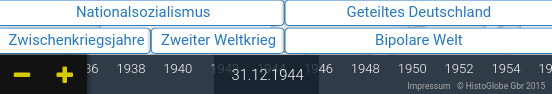
\includegraphics[width=0.8\textwidth]{graphics/timeline_now.png}
	\caption{Timeline}
\end{figure}

\subsubsection{Structure}
One requirement of the teacher is to present time in history not linear but in epochs. The advantage is that he can give focus to special subsets of history. In our implementation we have two different types of epoch bars: German history and world history.

So our actual implementation of the timeline consists of four layers. The top layer describes the German history from "Deutsches Kaiserreich" to "Geteiltes Deutschland". The next two layers belong together. They represent the world history from "Imperialismus" to "Bipolare Welt". The upper of these two layers is only shown if one category of the world history is selected. Like in picture ~\ref{fig:Timeline_Elements}. Here "Imperialismus" is active and on top of this layer is the subtopic layer with specific topics. The bottom line is used to show the classification of epoch in time and to show the certain moment of history in the DD.MM.JJJJ format as NowDate.

\begin{figure}[H]
	\centering
	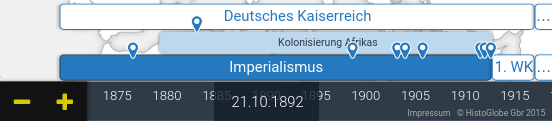
\includegraphics[width=0.8\textwidth]{graphics/timeline_elements.png}
	\caption{Timeline Elements}
	\label{fig:Timeline_Elements}
\end{figure}



\subsubsection{Behaviour}
The following section describes the individual functionalities of the Timeline and topic bars. All elements are linked together so if you change one element, all other elements are chained in the same way.

With the two control buttons on the left side you can \textbf{zoom} the time. We have limited the different displayed zoom levels to four steps (1, 2, 5, 10). These steps represent the distance of the displayed years. The date change if they begin to overlap the thresholds of each other. So you can zoom in and out and the Timeline is horizontal stretched or compressed.

To change the current date you can \textbf{pull} the Timeline. You can also move the Timeline by activate a Hivent. Then it is centered in the middle and the NowDate displays the date of the event.

One interesting task of the Epoch Bars was to \textbf{adapt} the labels \textbf{to different sizes}. In most cases the names of Epochs do not fit in their boxes. Therefore we tried different ways to fix this problem:

\begin{itemize}
	\item write epoch name in two lines (destroys layout)
	\item dynamic resize of Epoch Bars and no change of zoom level (historically incorrect because epochs overlap)
	\item dynamic resize of Epoch Bars and with adaption of zoom level (short historical epochs with long names destroys layout)
	\item leave out vowels (some epoch names are unreadable)
	\item leave out the middle of the word and replace it with ... (some epoch names are unreadable)
\end{itemize}

Finally, we have used a combination of two replacement rules like in Figure ~\ref{fig:Timeline_Elements2}:

\begin{enumerate}
	\item replace the entire word with an abbreviation
	\item replace the end of the word with ...
\end{enumerate}

To improve readability of the epoch names we placed it in the middle of the epoch boxes. If they come close to the edge they stick there with an threshold till the box box is to small.

\begin{figure}[H]
	\centering
	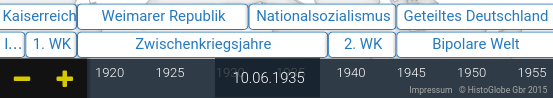
\includegraphics[width=0.8\textwidth]{graphics/timeline_elements2.png}
	\caption{Timeline Elements with all improvements}
	\label{fig:Timeline_Elements2}
\end{figure}

% subsection timeline (end)
